% !TeX TXS-program:compile = txs:///pdflatex/[--shell-escape]
% =========================================================================
\documentclass[notes, aspectratio=1610]{beamer}
%\documentclass[aspectratio=1610]{beamer}

% ========================= Theme =========================================
\usetheme{Berkeley}
\usecolortheme{seahorse}

% ========================= Essential packages ============================
\usepackage{hyperref}
\hypersetup{
    colorlinks = true,
    linkcolor = blue,
    citecolor = blue,
    filecolor = blue,
    urlcolor = blue
}

% ========================= Frame notes systm ============================
%\usepackage{pgfpages}
%\setbeameroption{show notes on second screen}

% ========================= Plotting ======================================
\usepackage{calc}
\usepackage{tikz}
\usetikzlibrary{arrows,
                arrows.meta,
                calc,
		chains,
                quotes,
                positioning,
		shapes,
                shapes.geometric}
\usepackage{graphicx}
\usepackage{graphics}
\usepackage{pgfplots}
\pgfplotsset{width=7cm,compat=1.17}

%% ============================== Tabular =================================
\usepackage{booktabs}
\usepackage{tabularx,ragged2e}
\usepackage{array}
\usepackage{multirow}
\usepackage{siunitx}
  \sisetup{detect-all}
\usepackage{adjustbox}
\usepackage{rotating}
\usepackage{threeparttable}
\usepackage[justification=centering]{caption}

%% ========================== Coding snippets =============================
% Default fixed font does not support bold face
\usepackage{minted}
\usemintedstyle{vs}

% ========================= Infor on authors ==============================
\title[What, how, and why of data viz]%
{The What, How, and Why of Data Visualization}
\subtitle{Data and Image Models}
\author{S.~Santoni\inst{1}\inst{2}}
\institute{
	\inst{1}%
	Bayes Business School
	\and
	\inst{2}%
	Soundcloud
	}
\date{MSc in Business Analytics, 2022/23}

% ============================ Colors =====================================
\definecolor{base_c}{rgb}{0.6,0,0}
\definecolor{comp_c}{rgb}{0.09803921568627451, 0.6901960784313725, 0.7529411764705882}
\definecolor{tri_1}{rgb}{0.09803921568627451, 0.7686274509803922, 0.19215686274509805}
\definecolor{tri_2}{rgb}{0.19215686274509805, 0.09803921568627451, 0.7686274509803922}

% ========================= TOC  ==========================================
%\AtBeginSubsection[]
%{
%	\begin{frame}
%		       \frametitle{Outline}
%		       \tableofcontents[currentsection,currentsubsection]
%	\end{frame}
%}

% ========================= References ===================================
\usepackage[style=numeric,backend=biber]{biblatex}
\addbibresource{bibliography.bib}

% =========================== TOC =========================================
\AtBeginSubsection[]
{
    \begin{frame}
        \frametitle{Outline}
        \tableofcontents[currentsection,currentsubsection]
    \end{frame}
}

% ========================= Document  ====================================
\begin{document}

\begin{frame}
	\titlepage
\end{frame}

\begin{frame}{Outline}
	\tableofcontents
\end{frame}

% ------------------------- Week 1 wrap up -----------------------------------
\section{Session \#1 Wrap Up}

\begin{frame}
	\frametitle{What are the `ingredients' of a data viz?}
		According to the designing thinking literature~\cite{ware2010}, 
		a data viz contains the following three groups of `ingredients:'
		\begin{itemize}
			\item
			User needs/benefits, i.e., the information 
			a user wants to achieve
			\item
			Design, i.e., the set of choices regarding the
			visual forms, color, density, redundancy, and so on
			that characterize a data viz
			\item
			Technology, i.e., the knowledge, tools, and 
			data underlying the data viz
		\end{itemize}
\end{frame}

\begin{frame}
	\frametitle{How does the data viz process look like?}
	\tikzstyle{decision} = [
		diamond,
		draw,  
		text width=8em,
		text centered, 
		node distance=2cm, 
		inner sep=0pt
		]
	\tikzstyle{block} = [
		rectangle, 
		draw,
		text width=8em,
		text centered,
		rounded corners,
		minimum height=2em
		]
	\tikzstyle{arrow} = [
		draw,
		-latex',
		rounded corners
		]
	\tikzstyle{line} = [
		draw
		]
	\tikzstyle{invisible4} = [
		rectangle
		]
	\tikzstyle{invisible5} = [
		rectangle
		]
	\tikzstyle{circular} = [
		draw,
		circle,
		radius=1.0cm,
		]

	The design thinking literature \cite{ware2010} suggests that the user
	needs/benefits component should be the starting point of the data viz process.
	The intuition is that data viz that addresses nobody's needs is useless!

	\vspace{1em}

	Instead, there is substantial flexibility when it comes to fix the design and 
	technology components. Ultimately, the order depends depends on contingent factors
	and the designer's background, skills, and preferences.

	\vspace{1em}

	\begin{columns}
		\begin{column}{0.45\textwidth}
			\emph{Pathway A}

			\vspace{1em}

			\begin{tikzpicture}[
				scale=0.8, every node/.style={scale=0.8},
				node distance = 1.5cm, auto, ->,
				]
				%% nodes
	                        \node [block] (nb) {\small Needs/benefits};
                                \node [block, below of = nb] (d) {Design};
                                \node [block, below of = d] (t) {Technology};
	                        %% arrows
	                        \path[]
	                        (nb) edge node [] {} (d)
	                        (d) edge node [] {} (t)
	                        \end{tikzpicture}
		\end{column}
		\begin{column}{0.45\textwidth}
			\emph{Pathway B}

			\vspace{1em}

			\begin{tikzpicture}[
				scale=0.8, every node/.style={scale=0.8},
				node distance = 1.5cm, auto, ->,
				]
				%% nodes
	                        \node [block] (nb) {\small Needs/benefits};
                                \node [block, below of = nb] (t) {Technology};
                                \node [block, below of = d] (d) {Design};
	                        %% arrows
	                        \path[]
	                        (nb) edge node [] {} (t)
	                        (t) edge node [] {} (d)
	                \end{tikzpicture}

		\end{column}
	\end{columns}
\end{frame}

\begin{frame}
	\frametitle{A closer understanding of the data viz process?}
	
	Do not worry!

	\vspace{2em}

	We will analyze the data viz process next week by the 
	`Data-Information-Knowledge-Wisdom' model~\cite{cairo2012}.	
\end{frame}

% =========================== Assignment ===================================
\section{Assignment Discussion}

\begin{frame}
    \frametitle{`The Good, the Bad, and the Ugly'}
    \begin{figure}
	\begin{small}
		\begin{center}
			
\includegraphics[width=0.4\textwidth]{
				images/goog_bad_ugly.jpg
				}
		\end{center}
	\end{small}
    \end{figure}
\end{frame}

% ============================ Graphical excellence =========================
\section{Graphical Excellence}

\begin{frame}
	\frametitle{What is a good data viz?}
	\begin{figure}
		\begin{small}
			\begin{center}
				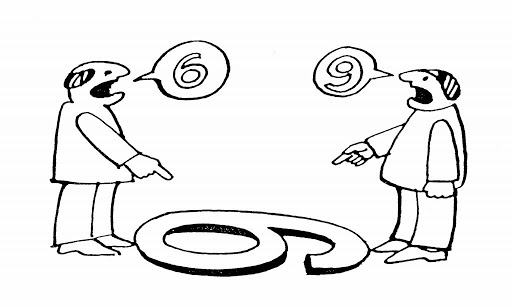
\includegraphics[width=0.95\textwidth]{images/subjectivity.jpg}
			\end{center}
		\end{small}
	\end{figure}
\end{frame}

\begin{frame}
	\frametitle{Example A: A Plot from the a Towards Data Science Post}
	\begin{figure}
		\begin{small}
			\begin{center}
				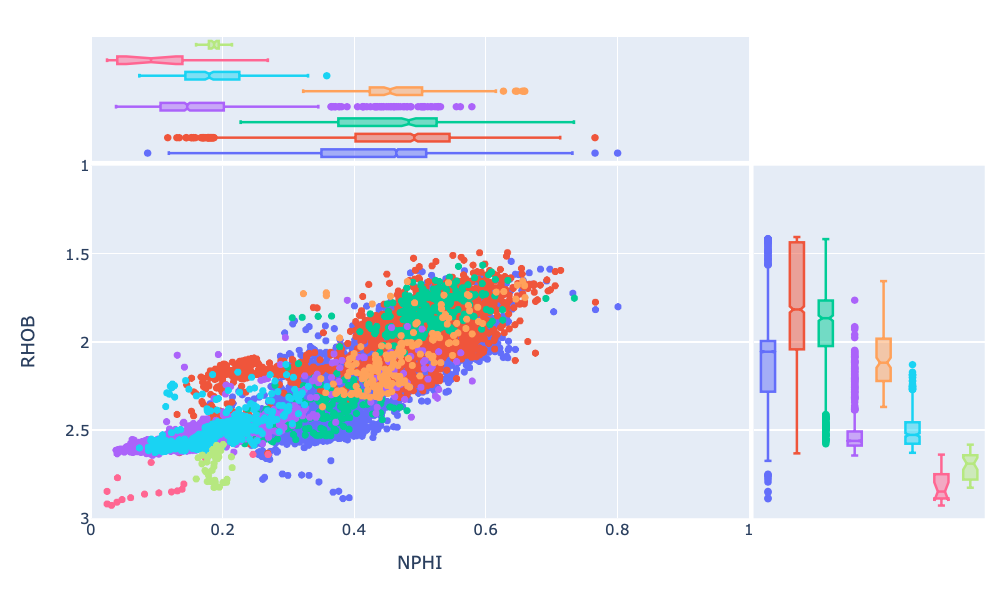
\includegraphics[width=0.9\textwidth]{images/plotly_scatter.png}
			\end{center}
		\end{small}
	\end{figure}

	\vspace{-1em}

	\footnotesize
	Source: \href{https://towardsdatascience.com/enhance-your-plotly-express-scatter-plot-with-marginal-plots-de469d42f12a}
	{https://towardsdatascience.com/enhance-your-plotly...}
\end{frame}

\begin{frame}
	\frametitle{Example B: A Chart from an Article in The Economist}
	\begin{figure}
		\begin{small}
			\begin{center}
				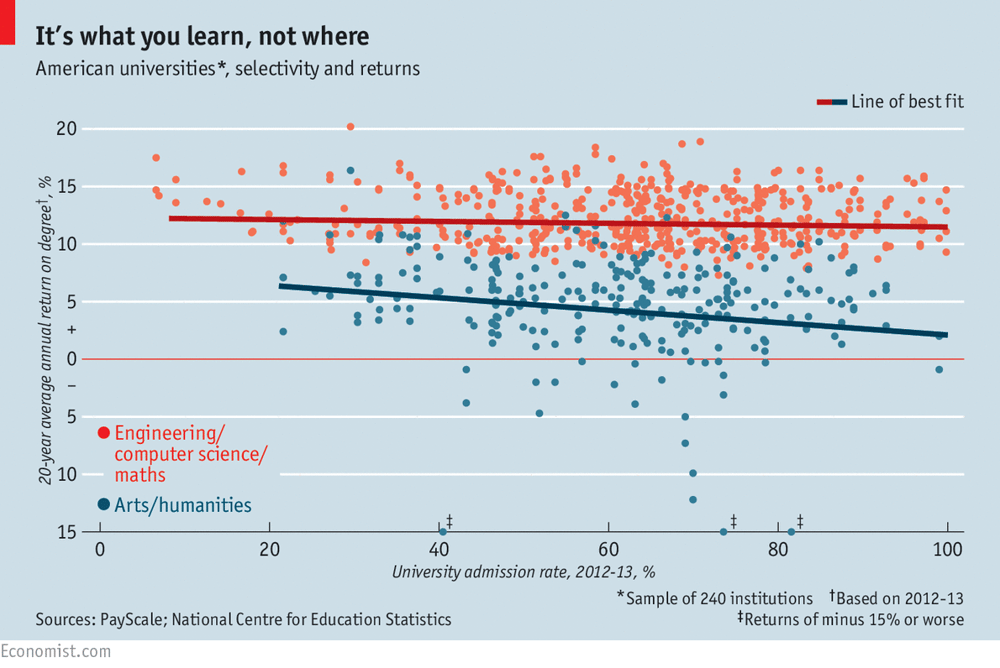
\includegraphics[width=0.75\textwidth]{images/economist_scatter.png}
			\end{center}
		\end{small}
	\end{figure}

	\footnotesize
	Source: \href{https://www.economist.com/united-states/2015/03/12/it-depends-what-you-study-not-where}
	{https://www.economist.com/...it-depends-what-you-study-not-where}
\end{frame}

\begin{frame}
	\frametitle{Graphical Excellence according to Tufte}
	Per Tufte's work \cite{tufte2001}, excellence in statistical graphs consists of complex 
	\emph{``ideas communicated with clarity, precision, and 
	efficiency.''}

	\vspace{1em}

	Graphical displays pursuing clarity, precision, and efficiency \emph{``
	give to the viewer the greatest number of ideas 
	in the shortest time with the least ink in the smallest space.''}

	\begin{figure}
		\begin{small}
			\begin{center}
				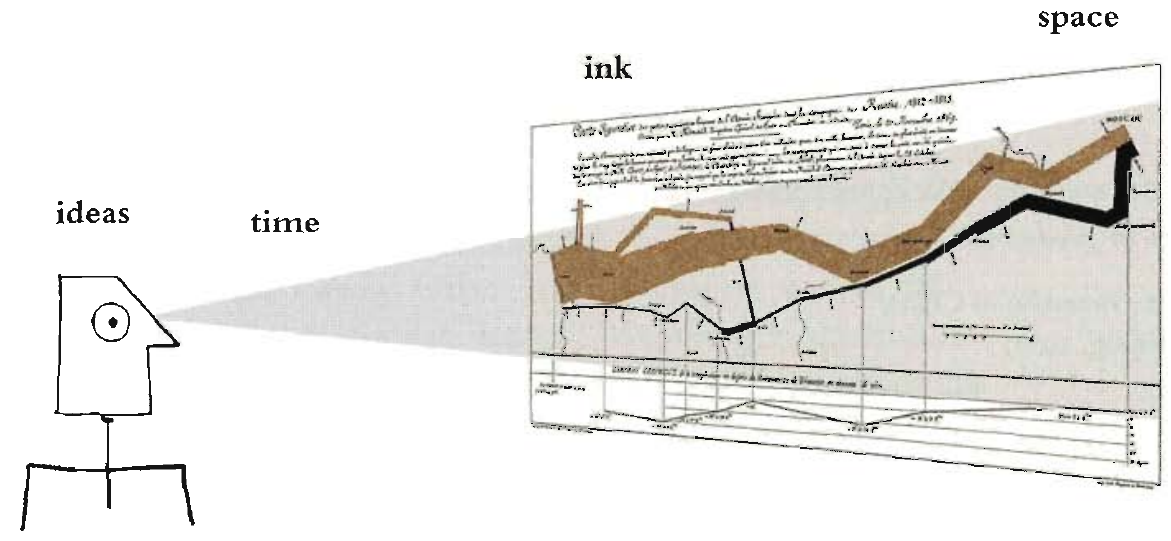
\includegraphics[width=0.85\textwidth]{
					images/graphical_excellence.png
					}
			\end{center}
			\caption{}
			\label{fig:}
		\end{small}
	\end{figure}
	
\end{frame}

\begin{frame}
	\frametitle{How to Reach Clarity, Efficiency, and Precision?}
	Tufte points out graphical displays should
	\begin{itemize}
		\item 
		Show the data
		\item 
		Induce the viewer to think about the substance rather than
		about the methodology, graphical design, the technology of 
		graphic production, or something else 
		\item 
		Avoid distorting what the data have to say 
		\item
		Present many number in a small space 
		\item 
		Make large datasets coherent
		\item
		Encourage the eye to compare different pieces of data 
		\item 
		Reveal the data at several levels of detail, from a broad 
		overview to the fine structure 
		\item 
		Serve a reasonably clear purpose: description, 
		exploration, tabulation, or decoration 
		\item 
		Be closely intergrated with the statistical and verbal 
		description of a data set 
	\end{itemize}
\end{frame}

\begin{frame}
	\frametitle{Show the Data!}
	Here is a classic example on the importance of showing the data, 
	the case of Anscombe's quartet \cite{anscombe1973}.

	\begin{figure}
		\begin{small}
			\begin{center}
				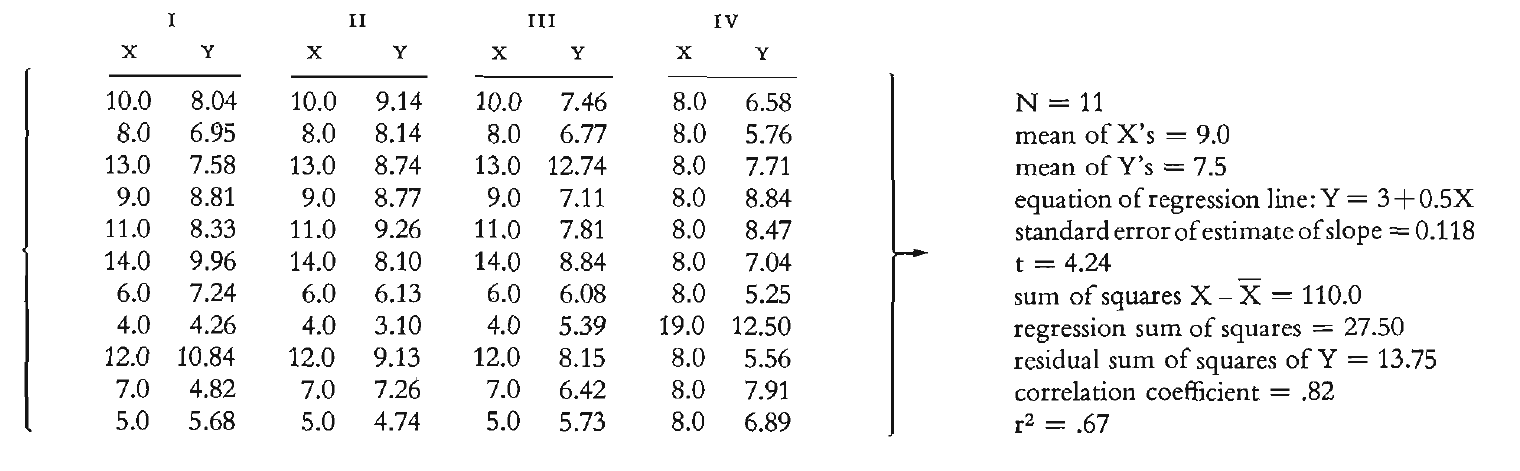
\includegraphics[width=1\textwidth]{
					images/anscombe_i.png
					}
			\end{center}
		\end{small}
	\end{figure}
	\footnote{See \cite[][page 14]{tufte2001}}
\end{frame}

\begin{frame}
	\frametitle{Show the Data! (cont'd)}
	\begin{figure}
		\begin{small}
			\begin{center}
				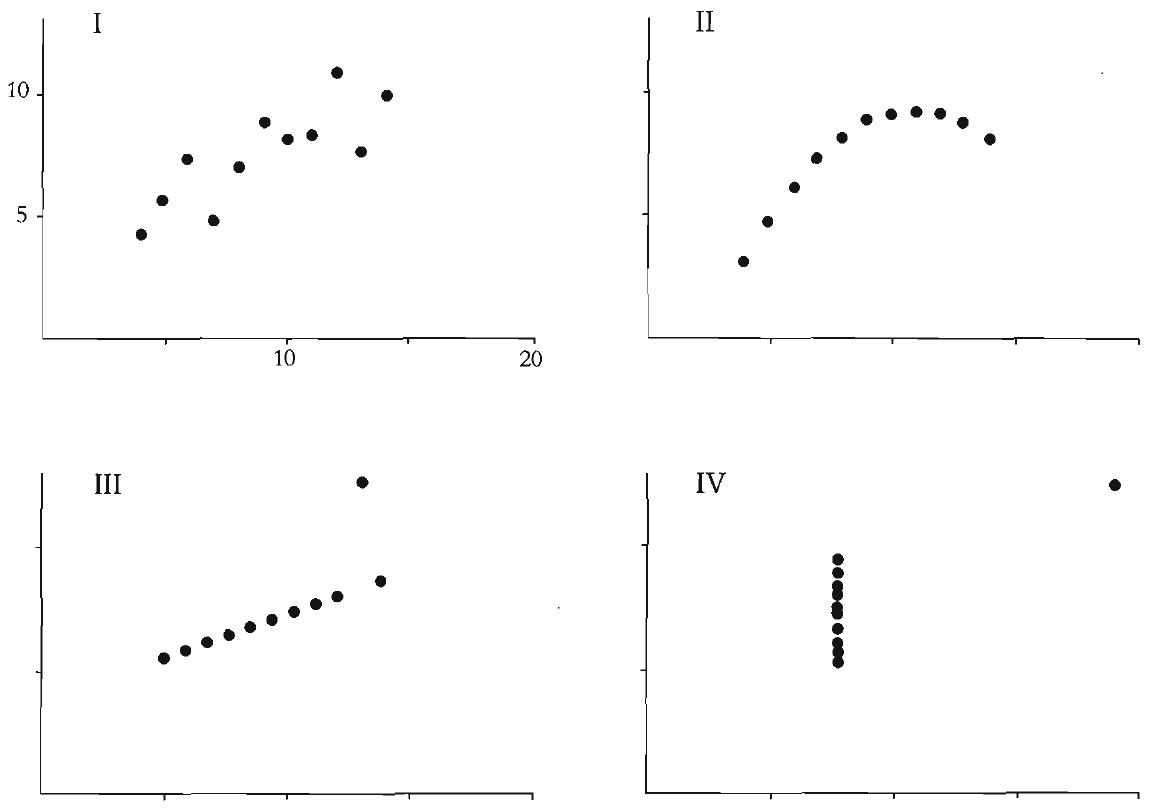
\includegraphics[width=0.80\textwidth]{
					images/anscombe_ii.png
					}
			\end{center}
		\end{small}
	\end{figure}
	
\end{frame}
% ============================ Graphical integrity =========================
\section{Graphical Integrity}

\begin{frame}
	\frametitle{...}
\end{frame}

% ======== Sources of integrity and sophistication =========================
\section{Sources of Integrity and Sophistication}

\begin{frame}
	\frametitle{...}
\end{frame}

% ========================== Session 2 wrap up =============================
\section{Session \#2 Wrap Up}

% =========================== Bibliography =================================

\begin{frame}
	\frametitle{References}
	\printbibliography
 \end{frame} 

\end{document}